\cleardoublepage
\chapter{ANALISIS MASALAH}
\label{chap:analisis-masalah}

Bab ini merupakan pelaksanaan fase identifikasi masalah dan definisi tujuan solusi dari metodologi \textit{Design Science Research} yang telah ditetapkan pada Subbab I.5.2. Pada fase identifikasi masalah, dilakukan observasi langsung terhadap kondisi pengelolaan sampah di Gedung Labtek VIII ITB untuk memahami permasalahan yang dihadapi. Pada fase definisi tujuan solusi, hasil observasi dirumuskan menjadi kebutuhan sistem, baik fungsional maupun nonfungsional. Bab ini ditutup dengan pemilihan alternatif solusi menggunakan metode AHP, yang menjadi titik transisi menuju fase perancangan dan pengembangan pada Bab IV, karena penetapan alternatif solusi terpilih merupakan masukan utama bagi perancangan artefak.

Bab ini menguraikan tiga aspek. Pertama, analisis kondisi saat ini yang mengidentifikasi permasalahan pengelolaan sampah akibat tidak adanya data terstruktur mengenai pola pembuangan. Kedua, analisis kebutuhan yang merumuskan spesifikasi sistem berdasarkan permasalahan yang ditemukan. Ketiga, pemilihan solusi melalui evaluasi alternatif untuk menentukan pendekatan yang paling sesuai dengan tujuan penelitian.

% ============================================================
\section{Analisis Kondisi Saat Ini}
\label{sec:analisis-kondisi}
% ============================================================

Berdasarkan observasi yang dilakukan di Gedung Labtek VIII, kondisi pengelolaan sampah saat ini bersifat konvensional. Tempat sampah tidak dilengkapi sensor atau sistem \textit{monitoring}, pengecekan dilakukan secara visual oleh petugas kebersihan, dan pengumpulan sampah dilakukan berdasarkan jadwal tetap tanpa mempertimbangkan kondisi aktual kepenuhan.

Dari kondisi tersebut, teridentifikasi tiga permasalahan utama:

\begin{enumerate}
    \item \textbf{Ketiadaan Data Terstruktur Mengenai Pola Pembuangan Sampah}

    Sistem pengelolaan sampah saat ini tidak memiliki mekanisme untuk mengumpulkan data mengenai pola pembuangan. Tidak ada informasi mengenai kapan puncak pembuangan terjadi, apakah ada perbedaan pola antara hari kerja dan akhir pekan, atau jenis sampah apa yang mendominasi. Pengambilan keputusan dilakukan tanpa basis data yang memadai.

    \item \textbf{Tidak Ada Dokumentasi Data Historis}

    Sistem saat ini tidak mendokumentasikan data pembuangan sampah dalam format yang terstruktur. Akibatnya, analisis tren jangka panjang, identifikasi perubahan pola seiring waktu, dan evaluasi efektivitas strategi pengelolaan tidak dapat dilakukan.

    \item \textbf{Pengelolaan Berdasarkan Jadwal Tetap tanpa Umpan Balik Data}

    Pengumpulan sampah dilakukan berdasarkan jadwal tetap dan pengecekan visual secara manual tanpa mempertimbangkan kondisi aktual kepenuhan sebelum pengecekan. Pendekatan ini berpotensi menyebabkan inefisiensi, yaitu pengumpulan dilakukan terlalu cepat saat tempat sampah masih kosong atau terlambat saat sudah penuh.
\end{enumerate}

Di sisi lain, perangkat \textit{Smart Waste Bin} berbasis IoT yang tersedia secara komersial umumnya dirancang untuk skala perkotaan. Konfigurasi bawaan perangkat, termasuk interval pengiriman data dan mekanisme pembacaan sensor pada \textit{firmware}, belum tentu sesuai untuk lingkungan yang lebih kecil seperti kampus, yang dinamika pembuangan sampahnya berubah dalam hitungan jam dan memerlukan titik data yang lebih tinggi. Hal ini menunjukkan bahwa selain membangun sistem pengumpulan data, diperlukan juga penyesuaian pada sisi \textit{firmware} perangkat agar dapat beroperasi secara optimal di lingkungan kampus.

Permasalahan tersebut menunjukkan bahwa pengelolaan sampah di lokasi pengujian masih berfungsi untuk keperluan dasar, namun tidak dilengkapi kemampuan untuk mengumpulkan dan menganalisis data mengenai pola pembuangan sampah. Kebutuhan akan sistem pemantauan sampah berbasis \textit{Internet of Things} yang disesuaikan, baik dari sisi perangkat lunak maupun \textit{firmware}, menjadi dasar analisis kebutuhan pada subbab berikutnya.

% ============================================================
\section{Analisis Kebutuhan}
\label{sec:analisis-kebutuhan}
% ============================================================

Analisis kebutuhan terbagi menjadi tiga bagian utama. Pertama, identifikasi pengguna sistem untuk memahami \textit{stakeholder} yang terlibat dan ekspektasi mereka terhadap sistem. Kedua, perumusan kebutuhan fungsional yang mendeskripsikan fungsi-fungsi spesifik yang harus dimiliki sistem. Ketiga, spesifikasi kebutuhan nonfungsional yang mendefinisikan karakteristik kualitas sistem.

\subsection{Identifikasi Pemangku Kepentingan}

Sebagai dasar untuk merumuskan kebutuhan sistem, dilakukan identifikasi pemangku kepentingan (\textit{stakeholder}) yang terkait dengan sistem pemantauan sampah berbasis \textit{Internet of Things}. Identifikasi ini bertujuan untuk memetakan pihak-pihak yang berkepentingan terhadap keluaran sistem sehingga kebutuhan fungsional dan nonfungsional dapat diturunkan secara tepat. Perlu ditegaskan bahwa kebutuhan sistem pada penelitian ini diturunkan dari permasalahan yang telah diidentifikasi, bukan dari pengujian terhadap pengguna. Pemangku kepentingan yang teridentifikasi adalah sebagai berikut:

\begin{enumerate}
    \item \textbf{Pengurus Lantai/Pengelola Gedung}

    Pengelola gedung berkepentingan terhadap pengawasan pengelolaan sampah dan pengambilan keputusan terkait strategi pengelolaan. Keluaran sistem yang relevan bagi pengelola gedung adalah informasi mengenai pola pembuangan sampah, tren volume sampah, dan \textit{insight} yang dapat mendukung perencanaan dan optimalisasi pengelolaan sampah.

    \item \textbf{Peneliti/Pengembang Sistem}

    Peneliti berkepentingan terhadap pengembangan, implementasi, dan \textit{maintenance} sistem. Keluaran sistem yang relevan meliputi ketersediaan \textit{raw data} untuk analisis, kemampuan konfigurasi sistem (seperti interval pembacaan sensor atau \textit{threshold}), dan \textit{interface} untuk \textit{monitoring} status operasional sistem.

    \item \textbf{Pengguna Gedung (\textit{Indirect Stakeholder})}

    Meskipun pengguna gedung (mahasiswa, dosen, \textit{staff}) tidak berinteraksi langsung dengan sistem, mereka merupakan sumber data pembuangan sampah. Keberadaan \textit{smart waste bin} tidak boleh mengubah atau mempersulit proses pembuangan sampah yang sudah berjalan.
\end{enumerate}

\subsection{Kebutuhan Fungsional}

Kebutuhan fungsional menjelaskan fungsi-fungsi dan fitur-fitur yang harus tersedia pada sistem. Berdasarkan identifikasi masalah dan kebutuhan pengguna, kebutuhan fungsional sistem pemantauan sampah berbasis \textit{Internet of Things} disajikan pada Tabel \ref{tab:kebutuhan-fungsional}.

\begin{longtable}{| l | l | p{4cm} | p{5cm} |}
  \caption{Kebutuhan Fungsional}
  \label{tab:kebutuhan-fungsional} \\
    \hline
    \textbf{ID} & \textbf{Komponen} & \textbf{Kebutuhan} & \textbf{Penjelasan} \\
    \hline
  \endfirsthead
    \hline
    \textbf{ID} & \textbf{Komponen} & \textbf{Kebutuhan} & \textbf{Penjelasan} \\
    \hline
  \endhead
    \hline
  \endfoot
    KF-01 & IoT \textit{Device} & Pembacaan Sensor & Sistem harus dapat membaca tingkat kepenuhan \textit{waste bin} menggunakan sensor dengan interval yang ditentukan \\
    \hline
    KF-02 & IoT \textit{Device} & Transmisi Data & Sistem harus dapat mengirimkan data ke \textit{server} melalui protokol komunikasi secara otomatis \\
    \hline
    KF-03 & IoT \textit{Device} & \textit{Time Stamping} & Setiap data harus dilengkapi \textit{timestamp} dan identifier \textit{waste bin} \\
    \hline
    KF-04 & IoT \textit{Device} & Konversi Data & Sistem harus dapat mengkonversi jarak hasil pembacaan sensor menjadi persentase kepenuhan (0--100\%) \\
    \hline
    KF-05 & \textit{Database} & Penyimpanan Data & Sistem harus dapat menyimpan data sensor secara terstruktur dan historis \\
    \hline
    KF-06 & \textit{Database} & Pengambilan Data & Sistem dapat menyediakan \textit{query} untuk mengambil data secara spesifik \\
    \hline
    KF-07 & Analisis & Analisis Pola Temporal & Sistem harus dapat mengidentifikasi pola pembuangan berdasarkan waktu (\textit{hourly}, \textit{daily}, \textit{weekly}) \\
    \hline
    KF-08 & Analisis & Statistik Deskriptif & Sistem harus dapat menghasilkan statistik deskriptif (\textit{mean}, median, std) untuk setiap pola \\
    \hline
    KF-09 & \textit{Dashboard} & Visualisasi Data & \textit{Dashboard} harus menampilkan status kepenuhan \textit{waste bin} terbaru \\
    \hline
    KF-10 & \textit{Dashboard} & Grafik Pola Temporal & \textit{Dashboard} harus menampilkan grafik pola pembuangan per jam, per hari, dan per minggu \\
    \hline
\end{longtable}

Tabel \ref{tab:mapping-rm-kf} menyajikan \textit{mapping} setiap kebutuhan fungsional dengan rumusan masalah pada Bab I.

\begin{table}[H]
  \caption{\textit{Mapping} Rumusan Masalah dengan Kebutuhan Fungsional}
  \label{tab:mapping-rm-kf}
  \begin{tabularx}{\textwidth}{| X | l |}
    \hline
    \textbf{Rumusan Masalah} & \textbf{Kebutuhan Fungsional} \\
    \hline
    RM-1: Rancangan dan implementasi sistem pemantauan sampah berbasis \textit{Internet of Things} (IoT) yang mampu mengumpulkan data secara periodik dan terstruktur & KF-01, KF-02, KF-03, KF-04, KF-05, KF-06 \\
    \hline
    RM-2: Pola pembuangan sampah yang dapat diidentifikasi berdasarkan data sistem dan validasinya terhadap observasi lapangan & KF-07, KF-08, KF-09, KF-10 \\
    \hline
  \end{tabularx}
\end{table}

\subsection{Kebutuhan Nonfungsional}

Kebutuhan nonfungsional mendeskripsikan karakteristik kualitas sistem yang harus dipenuhi, mencakup aspek performa, keandalan, dan akurasi, sebagaimana disajikan pada Tabel \ref{tab:kebutuhan-nonfungsional}.

\begin{table}[H]
  \caption{Kebutuhan Nonfungsional}
  \label{tab:kebutuhan-nonfungsional}
  \begin{tabularx}{\textwidth}{| l | l | X | X |}
    \hline
    \textbf{ID} & \textbf{Kategori} & \textbf{Kebutuhan} & \textbf{Penjelasan} \\
    \hline
    KNF-01 & \textit{Performance} & Waktu Pembacaan Sensor & Sensor harus dapat melakukan pembacaan dalam waktu maksimal 1 menit \\
    \hline
    KNF-02 & \textit{Performance} & Latensi Transmisi Data & Data harus dikirim ke \textit{server} dalam waktu maksimal 10 detik setelah pembacaan \\
    \hline
    KNF-03 & \textit{Performance} & \textit{Response Time Dashboard} & \textit{Dashboard} harus merespons interaksi pengguna dalam waktu maksimal 3 detik \\
    \hline
    KNF-04 & \textit{Performance} & Waktu \textit{Query} & \textit{Query} data dari \textit{database} harus selesai dalam waktu maksimal 5 detik \\
    \hline
    KNF-05 & \textit{Reliability} & \textit{Uptime} Sistem IoT & Sistem IoT harus beroperasi dengan \textit{availability} minimal 95\% \\
    \hline
    KNF-06 & \textit{Reliability} & Konsistensi Pembacaan & Pembacaan setiap 3 jam dengan toleransi keterlambatan maksimal $\pm$15 menit \\
    \hline
    KNF-07 & \textit{Reliability} & Kelengkapan Data & Minimal 90\% data harus berhasil dikumpulkan selama periode penelitian \\
    \hline
    KNF-08 & \textit{Accuracy} & Akurasi Sensor & Pembacaan sensor harus memiliki galat maksimal 10\% dari volume aktual \\
    \hline
  \end{tabularx}
\end{table}

% ============================================================
\section{Analisis Pemilihan Solusi}
\label{sec:analisis-solusi}
% ============================================================

Berdasarkan analisis kondisi saat ini dan kebutuhan sistem yang telah diidentifikasi, terdapat beberapa alternatif pendekatan dalam pengembangan sistem pemantauan sampah berbasis \textit{Internet of Things} (IoT). Bagian ini menguraikan alternatif-alternatif solusi yang dapat diterapkan serta analisis pemilihan solusi menggunakan metode \textit{Analytical Hierarchy Process} (AHP).

\subsection{Alternatif Solusi}

Berdasarkan analisis kebutuhan, seluruh alternatif solusi menggunakan perangkat \textit{Smart Waste Bin} yang tersedia dari pihak ketiga sebagai basis perangkat keras. Perbedaan antar alternatif terletak pada pendekatan \textit{software stack} untuk pengumpulan data, \textit{monitoring}, dan kemudahan \textit{maintenance} sistem. Analisis pola pembuangan (KF-07, KF-08) pada seluruh alternatif dilakukan melalui \textit{pipeline} analisis data terpisah menggunakan \textit{script} pengolahan data. Perlu dicatat bahwa setiap alternatif yang dipertimbangkan harus mampu memenuhi seluruh kebutuhan fungsional yang telah ditetapkan, termasuk KF-09 (\textit{monitoring} data terkini) yang mensyaratkan keberadaan antarmuka \textit{dashboard}; oleh karena itu, pendekatan tanpa \textit{dashboard} tidak dimasukkan sebagai alternatif karena sejak awal bertentangan dengan kebutuhan fungsional.

Terdapat dua alternatif solusi yang dapat diimplementasikan:

\begin{enumerate}
    \item \textbf{Alternatif 1: Perangkat \textit{Smart Waste Bin} + \textit{Platform Cloud} (ThingSpeak/Blynk)}

    Menggunakan perangkat \textit{Smart Waste Bin} dan mengintegrasikannya dengan \textit{platform} IoT \textit{cloud} untuk penyimpanan data dan visualisasi. Karakteristik alternatif ini: \textit{platform cloud} menyediakan \textit{backend} dan \textit{dashboard} siap pakai, \textit{deployment} cepat dengan konfigurasi minimal, namun fitur analisis terbatas pada yang disediakan \textit{platform} dan terdapat keterbatasan dalam \textit{custom query} untuk analisis pola temporal yang kompleks.

    \item \textbf{Alternatif 2: Perangkat \textit{Smart Waste Bin} + \textit{Backend Custom} + \textit{Dashboard}}

    Menggunakan perangkat \textit{Smart Waste Bin}, mengembangkan \textit{middleware} dan \textit{backend custom} (Supabase PostgreSQL), serta membangun \textit{dashboard} untuk \textit{monitoring}. Karakteristik alternatif ini: \textit{backend custom} memungkinkan \textit{query} fleksibel untuk analisis pola temporal, \textit{dashboard custom} untuk \textit{monitoring} status terkini dan visualisasi historis, dapat diintegrasikan dengan sistem lain, namun memerlukan \textit{effort} pengembangan \textit{middleware} dan \textit{dashboard}.
\end{enumerate}

Tabel \ref{tab:pemenuhan-kf} menyajikan pemenuhan kebutuhan fungsional untuk setiap alternatif solusi.

\begin{table}[H]
  \caption{Pemenuhan Kebutuhan Fungsional per Alternatif}
  \label{tab:pemenuhan-kf}
  \begin{tabularx}{\textwidth}{| X | l | l |}
    \hline
    \textbf{Kebutuhan} & \textbf{Alt-1} & \textbf{Alt-2} \\
    \hline
    KF-01 s.d. KF-04 (IoT \textit{Device}) & Terpenuhi & Terpenuhi \\
    \hline
    KF-05, KF-06 (\textit{Database}) & Terbatas & Terpenuhi \\
    \hline
    KF-07, KF-08 (Analisis Pola) & Terbatas & Terpenuhi \\
    \hline
    KF-09 (\textit{Monitoring} Terkini) & Terpenuhi & Terpenuhi \\
    \hline
    KF-10 (Visualisasi Historis) & Terbatas & Terpenuhi \\
    \hline
  \end{tabularx}
\end{table}

\subsection{Analisis Penentuan Solusi Menggunakan Metode AHP}

Untuk menentukan alternatif solusi yang paling sesuai, digunakan metode \textit{Analytical Hierarchy Process} (AHP). Metode ini dipilih karena dapat mengakomodasi kriteria-kriteria dengan bobot yang berbeda serta memberikan hasil yang terukur dan terstruktur.

\begin{figure}[H]
  \caption{Struktur Hierarki AHP Pemilihan Solusi}
  \label{fig:kriteria-ahp}
  \centering
  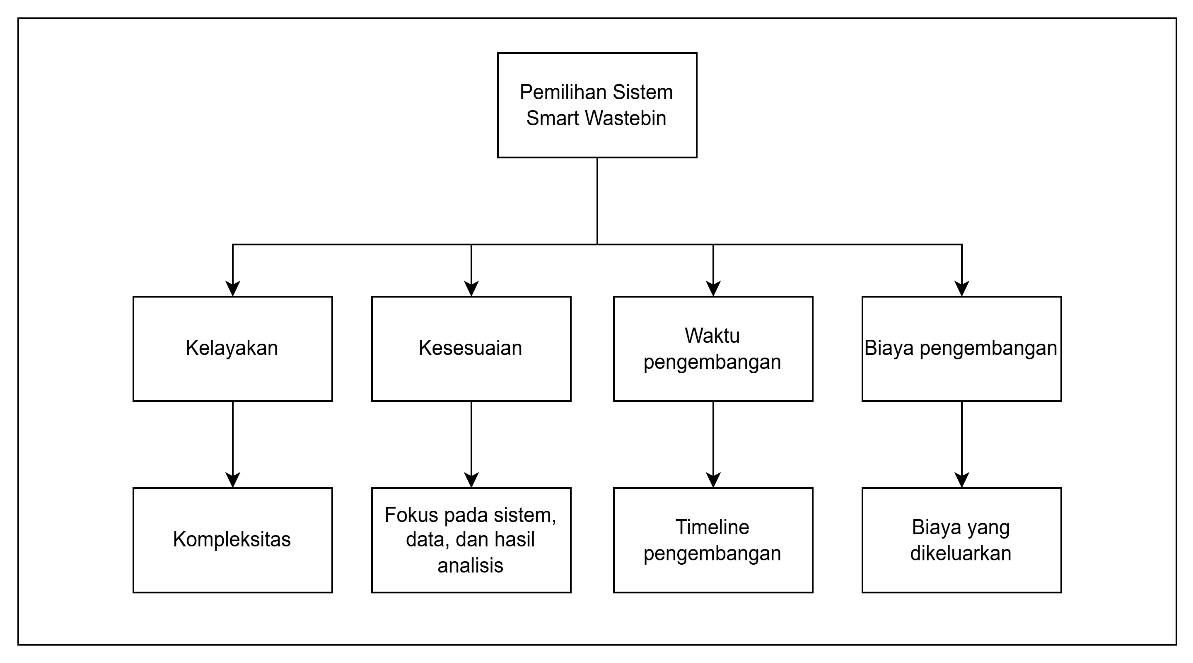
\includegraphics[width=0.9\textwidth]{images/kriteria-ahp.png}
  % RENAME: image6.png → kriteria-ahp.png di folder images/
\end{figure}

Gambar \ref{fig:kriteria-ahp} menunjukkan struktur hierarki AHP yang terdiri dari tujuan, kriteria, dan alternatif. Tabel \ref{tab:kriteria-ahp} menyajikan deskripsi setiap kriteria yang digunakan untuk evaluasi alternatif solusi.

\begin{table}[H]
  \caption{Kriteria Evaluasi Alternatif Solusi}
  \label{tab:kriteria-ahp}
  \begin{tabularx}{\textwidth}{| l | l | X |}
    \hline
    \textbf{ID} & \textbf{Kriteria} & \textbf{Deskripsi} \\
    \hline
    C-1 & Kelayakan Teknis & Kemudahan implementasi dengan kemampuan dan \textit{resource} yang tersedia \\
    \hline
    C-2 & Kesesuaian Tujuan & Seberapa baik solusi mendukung pencapaian tujuan penelitian (implementasi sistem, analisis pola, dan evaluasi \textit{firmware}) \\
    \hline
    C-3 & Waktu Pengembangan & Durasi waktu yang dibutuhkan untuk menyelesaikan pengembangan sistem \\
    \hline
    C-4 & Biaya & Total biaya implementasi yang dikeluarkan \\
    \hline
  \end{tabularx}
\end{table}

Penentuan bobot kriteria dilakukan melalui \textit{pairwise comparison matrix} menggunakan skala Saaty sebagaimana dijelaskan pada Subbab \ref{sec:ahp-teori}, dengan hasil disajikan pada Tabel \ref{tab:matriks-kriteria}. C-2 (Kesesuaian dengan tujuan penelitian) merupakan prioritas tertinggi karena sistem harus mendukung analisis pola dan evaluasi \textit{firmware}. C-1 (Kelayakan teknis) lebih penting dari C-3 (Waktu pengembangan). C-4 (Biaya) mendapat bobot terendah karena semua alternatif berada dalam \textit{range} biaya yang \textit{comparable}.

\begin{table}[H]
  \caption{Matriks Perbandingan Kriteria Berpasangan}
  \label{tab:matriks-kriteria}
  \begin{tabular}{| l | c | c | c | c |}
    \hline
    & \textbf{C-1} & \textbf{C-2} & \textbf{C-3} & \textbf{C-4} \\
    \hline
    \textbf{C-1} & 1     & 0,333 & 3     & 5 \\
    \hline
    \textbf{C-2} & 3     & 1     & 3     & 7 \\
    \hline
    \textbf{C-3} & 0,333 & 0,333 & 1     & 3 \\
    \hline
    \textbf{C-4} & 0,2   & 0,143 & 0,333 & 1 \\
    \hline
    \textbf{Jumlah} & 4,533 & 1,810 & 7,333 & 16 \\
    \hline
  \end{tabular}
\end{table}

Nilai perbandingan pada matriks menggunakan skala fundamental Saaty dengan nilai ganjil (1, 3, 5, 7, 9) yang merepresentasikan tingkat kepentingan: sama penting (1), sedikit lebih penting (3), lebih penting (5), sangat lebih penting (7), dan mutlak lebih penting (9), beserta nilai kebalikannya (resiprokal). Sebagai contoh, C-2 dinilai sedikit lebih penting dari C-1 (nilai 3) karena kesesuaian dengan tujuan penelitian merupakan prioritas tertinggi, sedangkan C-2 dinilai sangat lebih penting dari C-4 (nilai 7) karena seluruh alternatif memiliki struktur biaya yang serupa sehingga biaya bukan faktor pembeda yang signifikan.

Setelah proses normalisasi matriks dan perhitungan rata-rata baris, diperoleh bobot untuk setiap kriteria sebagaimana disajikan pada Tabel \ref{tab:bobot-kriteria}.

\begin{table}[H]
  \caption{Bobot Kriteria Hasil AHP}
  \label{tab:bobot-kriteria}
  \begin{tabular}{| l | c | c |}
    \hline
    \textbf{Kriteria} & \textbf{Bobot} & \textbf{Persentase} \\
    \hline
    C-1 (Kelayakan Teknis)   & 0,282 & 28,2\% \\
    \hline
    C-2 (Kesesuaian Tujuan)  & 0,515 & 51,5\% \\
    \hline
    C-3 (Waktu Pengembangan) & 0,145 & 14,5\% \\
    \hline
    C-4 (Biaya)              & 0,058 & 5,8\% \\
    \hline
  \end{tabular}
\end{table}

Nilai \textit{Consistency Ratio} (CR) dihitung untuk memastikan konsistensi penilaian. Dengan $\lambda_{max} = 4{,}141$, $CI = 0{,}047$, dan $RI = 0{,}90$, diperoleh $CR = 5{,}2\%$ yang berada di bawah batas 10\%, menunjukkan konsistensi yang baik.

\subsection{Evaluasi dan Pemilihan Alternatif Solusi}

Evaluasi dilakukan dengan membuat matriks perbandingan berpasangan untuk setiap kriteria terhadap kedua alternatif solusi. Tabel \ref{tab:justifikasi-kriteria} menyajikan justifikasi perbandingan untuk setiap kriteria.

\begin{table}[H]
  \caption{Justifikasi Perbandingan Alternatif pada Setiap Kriteria}
  \label{tab:justifikasi-kriteria}
  \begin{tabularx}{\textwidth}{| l | X |}
    \hline
    \textbf{Kriteria} & \textbf{Justifikasi Perbandingan} \\
    \hline
    C-1 (Kelayakan) & Alt-1 sedikit lebih unggul (nilai 3): \textit{platform} siap pakai dengan konfigurasi minimal, sedangkan Alt-2 memerlukan pengembangan \textit{middleware} dan \textit{dashboard} sendiri. \\
    \hline
    C-2 (Kesesuaian) & Alt-2 lebih unggul (nilai 5): memenuhi seluruh KF secara penuh, termasuk \textit{query} fleksibel untuk analisis pola temporal dan \textit{dashboard custom}; Alt-1 terbatas pada fitur analisis dan \textit{custom query} yang disediakan \textit{platform}. \\
    \hline
    C-3 (Waktu) & Alt-1 lebih unggul (nilai 5): \textit{plug-and-play} dengan waktu \textit{deployment} singkat, sedangkan Alt-2 memerlukan waktu pengembangan \textit{middleware} dan \textit{dashboard}. \\
    \hline
    C-4 (Biaya) & Setara (nilai 1): Alt-2 menggunakan layanan \textit{free tier} (Supabase, Vercel), sedangkan Alt-1 menggunakan \textit{platform} dengan \textit{tier} gratis yang tersedia; tidak ada perbedaan biaya yang signifikan. \\
    \hline
  \end{tabularx}
\end{table}

Karena perbandingan hanya melibatkan dua alternatif, setiap matriks perbandingan berukuran $2 \times 2$ yang secara matematis selalu konsisten ($CR = 0\%$). Tabel \ref{tab:bobot-lokal} menyajikan bobot lokal untuk setiap alternatif pada setiap kriteria hasil normalisasi matriks perbandingan berpasangan.

\begin{table}[H]
  \caption{Bobot Lokal Alternatif pada Setiap Kriteria}
  \label{tab:bobot-lokal}
  \begin{tabular}{| l | c | c | c | c |}
    \hline
    \textbf{Alternatif} & \textbf{C-1} & \textbf{C-2} & \textbf{C-3} & \textbf{C-4} \\
    \hline
    Alt-1: SWB + \textit{Platform Cloud}       & 0,750 & 0,167 & 0,833 & 0,500 \\
    \hline
    Alt-2: SWB + \textit{Backend} + \textit{Dashboard} & 0,250 & 0,833 & 0,167 & 0,500 \\
    \hline
  \end{tabular}
\end{table}

Skor global dihitung dengan mengalikan bobot lokal dengan bobot kriteria, sebagaimana disajikan pada Tabel \ref{tab:skor-global}.

\begin{table}[H]
  \caption{Skor Global untuk Setiap Alternatif Solusi}
  \label{tab:skor-global}
  \begin{tabularx}{\textwidth}{| X | l | c | c |}
    \hline
    \textbf{Alternatif} & \textbf{Perhitungan} & \textbf{Skor} & \textbf{\%} \\
    \hline
    Alt-1: SWB + \textit{Platform Cloud}       & $\Sigma(\text{bobot lokal} \times \text{bobot kriteria})$ & 0,447 & 44,7\% \\
    \hline
    Alt-2: SWB + \textit{Backend} + \textit{Dashboard} & $\Sigma(\text{bobot lokal} \times \text{bobot kriteria})$ & 0,553 & 55,3\% \\
    \hline
  \end{tabularx}
\end{table}

Berdasarkan Tabel \ref{tab:skor-global}, Alternatif 2 terpilih sebagai solusi terbaik dengan skor 0,553 (55,3\%), unggul dibandingkan Alternatif 1 (44,7\%). Keunggulan Alternatif 2 berasal dari dominasi pada kriteria C-2 (Kesesuaian dengan tujuan penelitian) yang memiliki bobot tertinggi (51,5\%), dengan kontribusi sebesar $0{,}833 \times 0{,}515 = 0{,}429$ terhadap skor globalnya. Meskipun Alternatif 1 unggul pada kelayakan teknis (C-1) dan waktu pengembangan (C-3), keterbatasan fitur analisis dan \textit{custom query} pada \textit{platform cloud} menyebabkan skor C-2 yang rendah, padahal kemampuan analisis pola temporal merupakan inti dari tujuan penelitian ini.

Dengan demikian, sistem pemantauan sampah berbasis \textit{Internet of Things} akan diimplementasikan menggunakan Alternatif 2, yaitu perangkat \textit{Smart Waste Bin} dari pihak ketiga dengan \textit{backend custom} (Supabase) dan \textit{dashboard} untuk \textit{monitoring}. Analisis pola pembuangan dilakukan melalui \textit{pipeline} analisis data terpisah. Selain pengembangan \textit{software stack}, adaptasi pada sisi \textit{firmware} perangkat juga akan dilakukan untuk menyesuaikan konfigurasi bawaan yang dirancang untuk skala perkotaan agar optimal di lingkungan kampus, sebagaimana telah diidentifikasi pada Subbab \ref{sec:analisis-kondisi}.